\section{Theoretical Analysis}
\label{sec:analysis}

Because our input voltage was $Vs = 230V$, and the expected output voltage was 12V, a transformer was used to convert Vs into a smaller value, given by the expression $Vr=Vs/n$, with $n=10$. On its own, however, this step doesn't solve the whole problem, as the objective of this assignment is to make an AC/DC Converter Circuit. So, we still need to convert the transformed AC voltage into a DC voltage. To do this, the circuit shown in Figure~\ref{fig:cir} was used.

This circuit is composed by three main subcircuits. 

The four diodes on the left make up the Full-wave Rectifier. This subcircuit is responsible for transforming the AC voltage into an equal amplitude but unidirectional voltage, as shown in green, in Figure~\ref{fig:output}. This can be computed by simply taking the absolute value of the transformed voltage vr. 

After that, a capacitor is utilized to reduce the magnitude of the voltage, getting it even closer to a DC voltage, as shown in COLOR, in Figure~\ref{fig:output}. This can be computed by determining when the diodes are ON an OFF. Periodically, we get:

\begin{equation}
    \begin{cases}
        vO = Vr \qquad , t < t_{OFF} \\
	    vO = Vs \cdot cos(w \cdot t_{OFF}) \cdot exp(-\frac{t-t_{OFF}}{R_{eq} \cdot C}) \qquad , t > t_{OFF}.
    
  \label{eq:vo}  
  \end{cases}
\end{equation}


Finally, 22 diodes in series are used for the purpose of reducing the noise, making the plot even closer to DC, as shown in COLOR, in Figure~\ref{fig:output}. By calculating the vO average, one can see if the voltage drop at the diodes terminals is limited by the maximum voltage that those diodes can handle. This is the case when that average is greater than that maximum. After this, we are left with a voltage due to the DC component, so we still need to take into account the AC component. This can be computed by calculating rd (the resistance of each diode), which depends on the diode material properties.

Then, the AC component is given by:

$vO_{AC} = number of diodes \cdot \frac{rd}{number of diodes \cdot rd+R2} \cdot (vO_{envelope}-average_{envelope})$

With this, vO is simply given by: $vO$ = $vO_{DC}$ + $vO_{AC}$.

This value should be close to 12V.

\begin{table}[ht]
  \centering
  \begin{tabular}{|l|r|}
    \hline    
    {\bf Name} & {\bf Value} \\ \hline
	enveloperipple & 2.562498e-01 \\ \hline
envelopeaverage & 1.424920e+01 \\ \hline

  \end{tabular}
  \caption{Ripple and average envelope values}
	\label{tab:envelope}
\end{table}

\begin{table}[ht]
  \centering
  \begin{tabular}{|l|r|}
    \hline    
    {\bf Name} & {\bf Value} \\ \hline
        regulatorripple & 6.729519e-02 \\ \hline
regulatoraverage & 1.200000e+01 \\ \hline

  \end{tabular}
  \caption{Ripple and average regulator values} 
        \label{tab:regulator}
\end{table}     





\begin{figure}[h] \centering
\includegraphics[width=0.6\linewidth]{output.eps}
	\caption{Transformed input voltage, vr, Envelope Detector and Voltage Regulator output voltages}
	\label{fig:output}
\end{figure}

\begin{figure}[h] \centering                                          
\includegraphics[width=0.6\linewidth]{ac_component.eps}          
	\caption{Envelope detector and voltage regulator output voltages deviations around 12V}                                   
        \label{fig:ac_dc}                                            
\end{figure}








